\documentclass[9pt,twocolumn,twoside]{../../styles/osajnl}
\usepackage{fancyvrb}
\journal{i524} 

\title{Hive}

\author[1,*, +]{Diksha Yadav}

\affil[1]{School of Informatics and Computing, Bloomington, IN 47408, U.S.A.}

\affil[*]{Corresponding authors: yadavd@umail.iu.edu}

\affil[+]{HID - S17-IR-2044}

\dates{Paper-002, \today}

\ociscodes{Hive, Hadoop, HiveQL, SQL, HDFC, RDBMS}

% replace this with your url in github/gitlab
\doi{\url{https://github.com/cloudmesh/sp17-i524/tree/master/paper2/S17-IR-2044/report.pdf}}


\begin{abstract}
Hive is an open source data warehousing solution which is built on top of Hadoop. It structures data into understandable and conventional database terms like tables, columns, rows and partitions. It supports HiveQL queries which have structure like SQL queries. HiveQL queries are compiled to map reduce jobs which are then executed by Hadoop. Hive also contains Metastore which includes schemas and statistics which is useful in query compilation, optimization and data exploration.

\end{abstract}

\setboolean{displaycopyright}{true}

\begin{document}

\maketitle

\section{Introduction}
Hive is an ETL and open source data warehousing solution which is built on top of Hadoop Distributed File System. Hive was built in January 2007 and open sourced in August 2008.
 It structures data into understandable and conventional database terms like tables, columns, rows and partitions. It supports HiveQL queries which have structure like SQL queries. HiveQL queries are compiled to map reduce jobs which are then executed by Hadoop. Hive also contains Metastore which includes schemas and statistics which is useful in query compilation, optimization and data exploration. In short, hive can be used by analyzing huge datasets, performing encapsulation of data and running ad hoc queries \cite{wk}

\section{Architecture}
Hive architecture as provided in Fig.1. from \cite{td} has, 
Database-It consists of tables created by the user.
Hadoop Distributed File System and or Hbase are used as data storage techniques to store data in file system.
Metastore-It contains information about the system. It can be accessed by different components as and when needed. All components of hive interact with metastore
Interfaces-User interface and Application programming interface both are present in hive.
External interfaces which includes Command Line Interface Web User Interface. Also it contains JDBC and ODBC Application programming Interfaces
Driver-manage HiveQL statements at every stage which includes compilation stage, optimization stage and execution stage. A session handle is created every time a Hive QL statement is received from any interfaces or thrift server which records information like number of output rows , execution time etc.
Query compiler-It compiles HiveQL queries to acyclic graphs (directed) representing map reduce tasks.
Execution Engine- It executes the tasks generated by the compiler.
Hive Server- It provide JDBC/ODBC server and thrift interface.
Compiler-When a Hive QL statement is received from interface, the driver invokes the compiler for performing its task of translating the Hive QL statement into Directed acyclic graph of map reduce jobs.
The map reduce jobs are then submitted by the driver to execution engine (like Hadoop) in a topological order \cite{td}

\begin{figure}[htbp]
	\centering
	\fbox{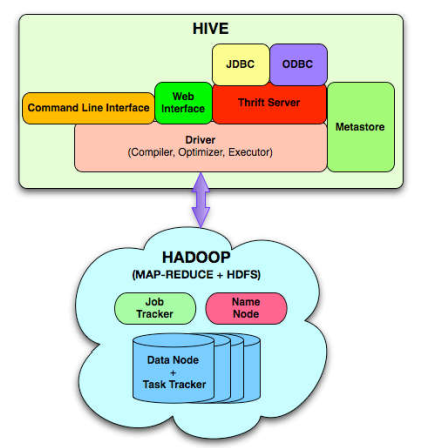
\includegraphics[width=\linewidth]{images/harch.png}}
	\caption{Hive Architecture}
	\label{fig:Hive-arch}
\end{figure} 

\section{QUERY EXECUTION IN HIVE}
When a query is submitted to the hive.
Compiler compiles the query.
The compiled query is executed by execution engine like MapReduce.
Resources are then allocated across the clusters for application by the resource manager, YARN.
The data that is used by the query is stored in HDFS (Hadoop Distributed File System). Supported data formats are AVRO, Parquet, ORC and text.\newline
When results from query are ready, they are set back using JDBC/ODBC connection.
\cite{ht}


\section{Features}
Hive can be used with structured or semi structured data only.\newline
HiveQL does not require user to deal with MapReduce complex programming. \newline
Infact user has to use concepts similar to relational database like tables, schema, rows, columns etc.\newline
Hive supports four file formats, text file, sequence file, orc and rcfile.\newline
HiveQL syntax is similar to SQL syntax.\newline
Hive query executes on Hadoop’s infrastructure rather than traditional database.\newline
Hive uses partition concept for data retrieval.\newline
Hive supports custom User defined functions for data cleansing, filtering etc. \newline
Hive can be used in two modes, local mode and MapReduce mode.\newline
Selection of mode depends on certain conditions like data size, data nodes in Hadoop.\newline
By default, hive runs on MapReduce mode.\newline
\cite{gr}

\section{System Requirements}
Hive is cross platform. So, It does not need any specific operating system to work.\newline
Minimum System Requirements:\newline
CPU Speed:Intel Dual-Core 2.4 GHz or AMD equivalent\newline
RAM:2 GB\newline
OS:Windows 7\newline
Video Card:NVIDIA GeForce 8800GT\newline
Sound Card:DirectX®-compatible\newline
Free Disk Space:1 GB\newline
Prefered System Requirements:\newline
CPU Speed:Intel Dual-Core 2.4 GHz or AMD equivalent\newline
RAM:4 GB\newline
OS:Windows 7\newline
Video Card:NVIDIA GeForce GTX 260\newline
Sound Card:DirectX®-compatible\newline
Free Disk Space:1 GB\newline \cite{sr}

\section{Comparison of Hive with Other Traditional Databases}
Traditional databases like RDBMS follow schema on write approach that is read and write many times while Hive follows schema on read approach that is write once and read many times.\newline
In schema on write, databases checks at load time if the data follows the table representation given by user while in schema on read approach, it is checked at run time only. This saves the time for hive to load the data when traditional databases takes longer time.  \newline
Hive does not support record level updates like RDMS. For example, we cannot perform delete, update, insert etc at record level in hive like we can perform in RDBMS.\newline
Hive does not support OLTP (Online Transaction Processing), it only supports OLAP (Online Analytical Processing) whereas RDBMS supports both OLTP and OLAP.\newline
For dynamic data analysis, RDMS would be preferred if quick responses are needed. Hive is suitable for data warehousing applications, where analysis is done on static data and fast responses are not needed. \newline
One more difference between hive and RDBMS is that hive is scalable and that too at low cost, while scalability comes at higher cost in RDBMS.\cite{p2}

\section{Popularity of Hive}
The popularity of hive is increasing with time. This can be proved by the following plot made by DB Engines Ranking. It ranks database management systems according to their status and popularity.
Following plot shows popularity of hive with time.

\begin{figure}[htbp]
	\centering
	\fbox{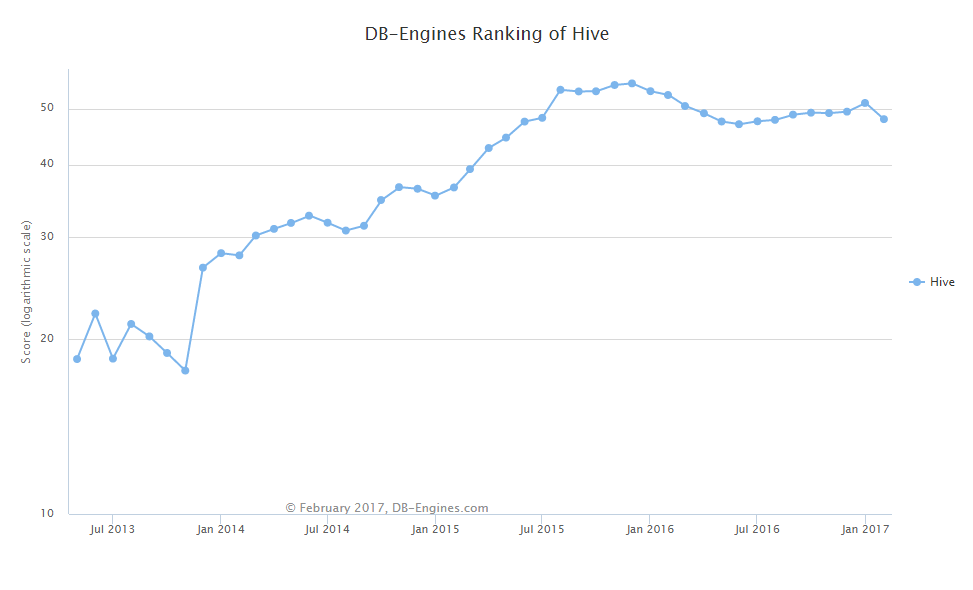
\includegraphics[width=\linewidth]{images/hgraph.png}}
	\caption{Hive Popularity}
	\label{fig:HivePopularity}
\end{figure}
\cite{rank}

\section{Resources for learning Hive}
Someone new to hive can start learning it by going through the following links in sequence:
Install Hive\url{https://www.edureka.co/blog/apache-hive-installation-on-ubuntu?utm_source=quora&utm_medium=crosspost&utm_campaign=social-media-edureka-ab}\newline
Hive Tutorial\url{https://www.edureka.co/blog/hive-tutorial/?utm_source=quora&utm_medium=crosspost&utm_campaign=social-media-edureka-ab}\newline
Top Hive commands with examples\url{https://www.edureka.co/blog/hive-commands-with-examples?utm_source=quora&utm_medium=crosspost&utm_campaign=social-media-edureka-ab}\newline

\section{Acknowledgement}
I am also grateful to Dr. Gregor von Laszewski for providing the appropriate paper template.


\section{Conclusion}
Hive is an ETL and data warehouse tool on top of Hadoop framework which is used for processing structured and semi structured data.\newline
Hive provides flexible query language such as HiveQL for querying and processing of data.\newline
It makes working easier for the user as they do not have to deal with MapReduce programming complexity when using SQL like structure of HiveQL\newline
It provides many new and better features compared to RDMS which has certain limitations.\newline
It supports writing and deploying custom user defined scripts and User defined functions.\newline


% Bibliography

\bibliography{references}

\end{document}
